\section{Expériences comparatives}
\label{sec:experiences}

\subsection{Protocole expérimental}

Un benchmark ciblé a été exécuté avec le moteur AUSSI V2 sur deux labyrinthes
(simple et pondéré), un trajet routier, un 8-Puzzle moyen et deux instances
arithmétiques (cible 24 et cible impossible 99). Les quatre stratégies
\BFS{}, \UCS{}, \Greedy{} et \AStar{} ont été évaluées. Les deux modes
\TreeSearch{} et \GraphSearch{} ont été comparés pour les labyrinthes; les
autres problèmes ont été exécutés en \GraphSearch{}. Une expérience
complémentaire compare, sur le même 8-Puzzle, trois heuristiques avec \AStar{} :
heuristique nulle, tuiles mal placées et distance de Manhattan.

Le jeu de données contient 44 exécutions. Pour chacune, le CSV conserve le
statut de résolution, le coût et la profondeur lorsqu'une solution est trouvée,
les noeuds générés et expansés, la taille maximale de \code{OPEN} et le temps
mesuré. \code{max\_open} est la taille maximale de la frontière; ce n'est pas
une mesure de la mémoire totale du processus. Chaque temps correspond à une
exécution unique et doit être interprété comme indicatif. Les nombres de noeuds
sont plus appropriés aux comparaisons reproductibles.

\subsection{Stratégies et gestion des états répétés}

La \cref{tab:maze-weighted} donne les résultats complets sur le labyrinthe
pondéré. Toutes les stratégies trouvent ici une solution de coût 9 et de
profondeur 6. Cette instance particulière ne départage donc pas les stratégies
sur le coût, mais met en évidence l'effet du mode de recherche sur l'effort.

\begin{table}[H]
\centering
\caption{Résultats sur le labyrinthe pondéré.}
\label{tab:maze-weighted}
\scriptsize
\begin{tabular}{llrrrrrr}
\toprule
\textbf{Stratégie} & \textbf{Mode} & \textbf{Gén.} & \textbf{Exp.} &
\textbf{OPEN max.} & \textbf{Coût / prof.} & \textbf{Résolue} &
\textbf{Temps (s)} \\
\midrule
BFS & Graphe & 32 & 13 & 3 & 9 / 6 & Oui & 0,000052 \\
BFS & Arbre & 203 & 85 & 118 & 9 / 6 & Oui & 0,000389 \\
UCS & Graphe & 37 & 15 & 3 & 9 / 6 & Oui & 0,000064 \\
UCS & Arbre & 1\,442 & 596 & 846 & 9 / 6 & Oui & 0,007855 \\
Greedy & Graphe & 23 & 9 & 4 & 9 / 6 & Oui & 0,000104 \\
Greedy & Arbre & 26 & 10 & 16 & 9 / 6 & Oui & 0,000162 \\
A* & Graphe & 30 & 12 & 5 & 9 / 6 & Oui & 0,000089 \\
A* & Arbre & 79 & 31 & 48 & 9 / 6 & Oui & 0,000189 \\
\bottomrule
\end{tabular}
\end{table}

\begin{figure}[H]
\centering
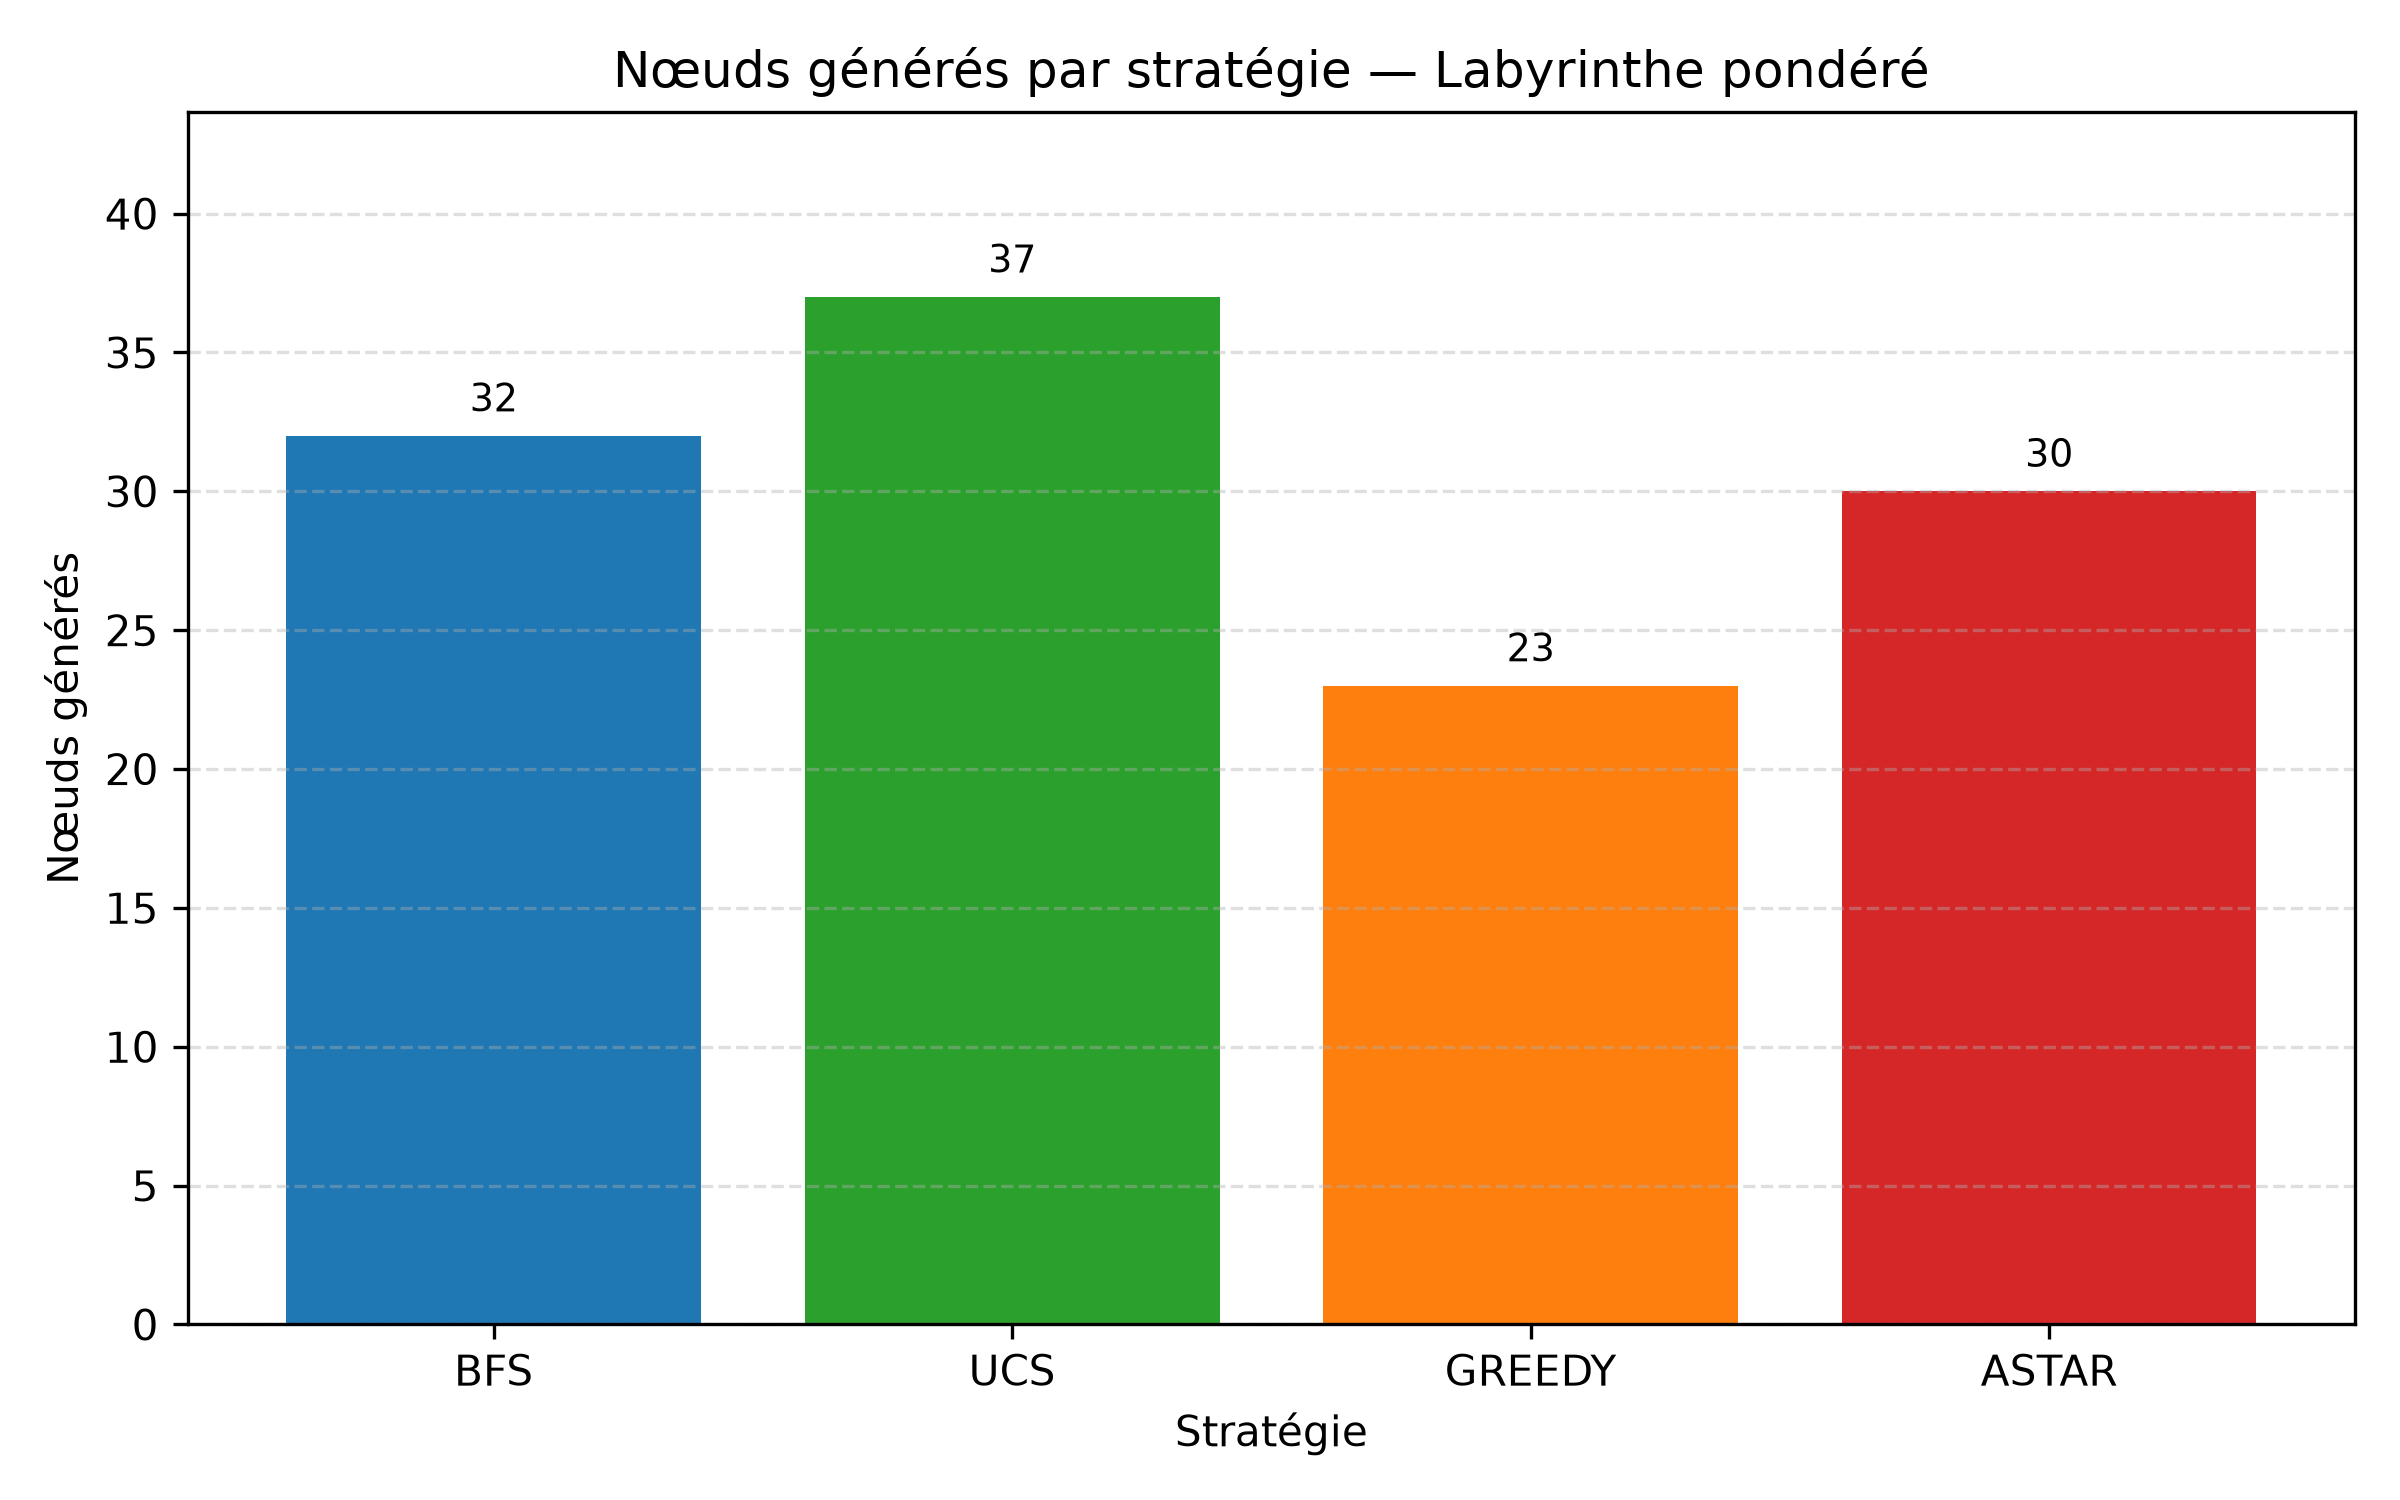
\includegraphics[width=0.78\textwidth]{figures/strategies_noeuds.png}
\caption{Noeuds générés par stratégie sur le labyrinthe pondéré en
\GraphSearch{}.}
\label{fig:strategies-noeuds}
\end{figure}

\begin{figure}[H]
\centering
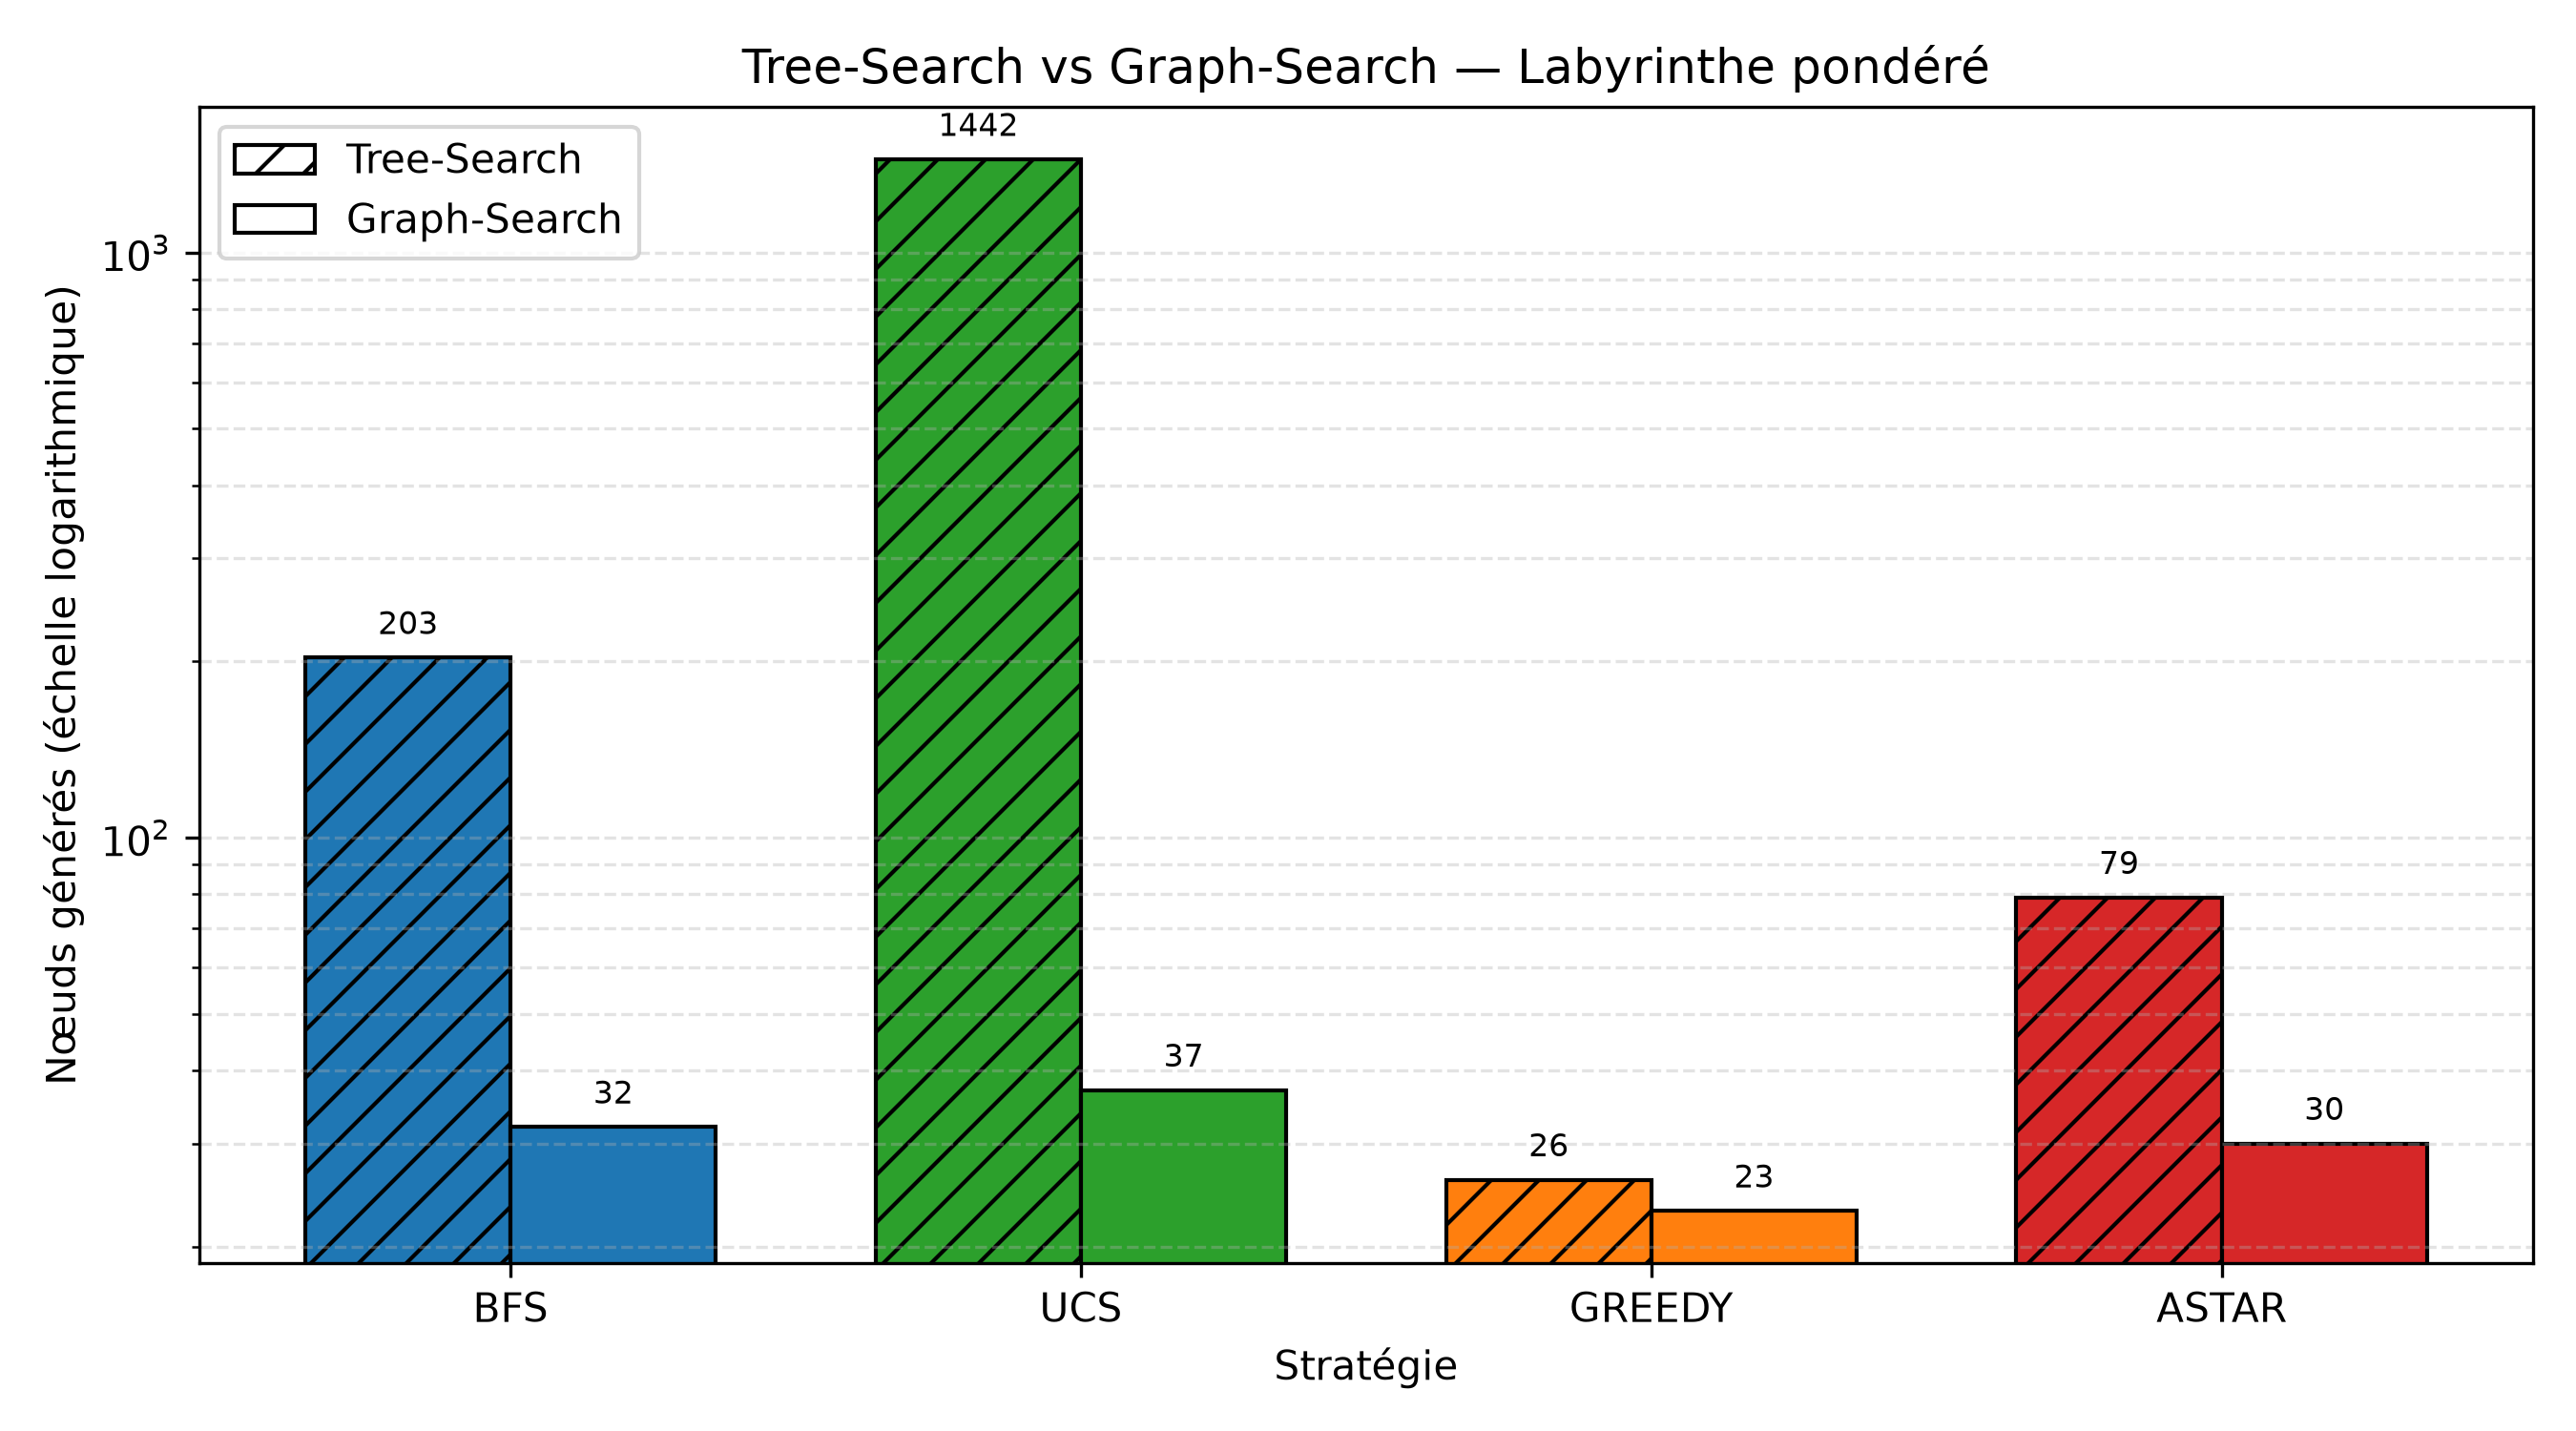
\includegraphics[width=0.82\textwidth]{figures/tree_vs_graph.png}
\caption{Noeuds générés en recherche arbre et graphe sur le labyrinthe
pondéré. L'axe vertical est logarithmique.}
\label{fig:tree-vs-graph}
\end{figure}

Sur ce labyrinthe, \GraphSearch{} réduit les noeuds expansés de 84,7\,\% pour
\BFS{} et de 97,5\,\% pour \UCS{}, par rapport à \TreeSearch{}. Pour Greedy, la
réduction est de 10,0\,\%, et pour \AStar{}, de 61,3\,\%. Le résultat dépend de
l'instance : sur le labyrinthe simple, les réductions correspondantes sont
respectivement de 50,0\,\%, 71,4\,\%, 0\,\% et 0\,\%.

\begin{figure}[H]
\centering
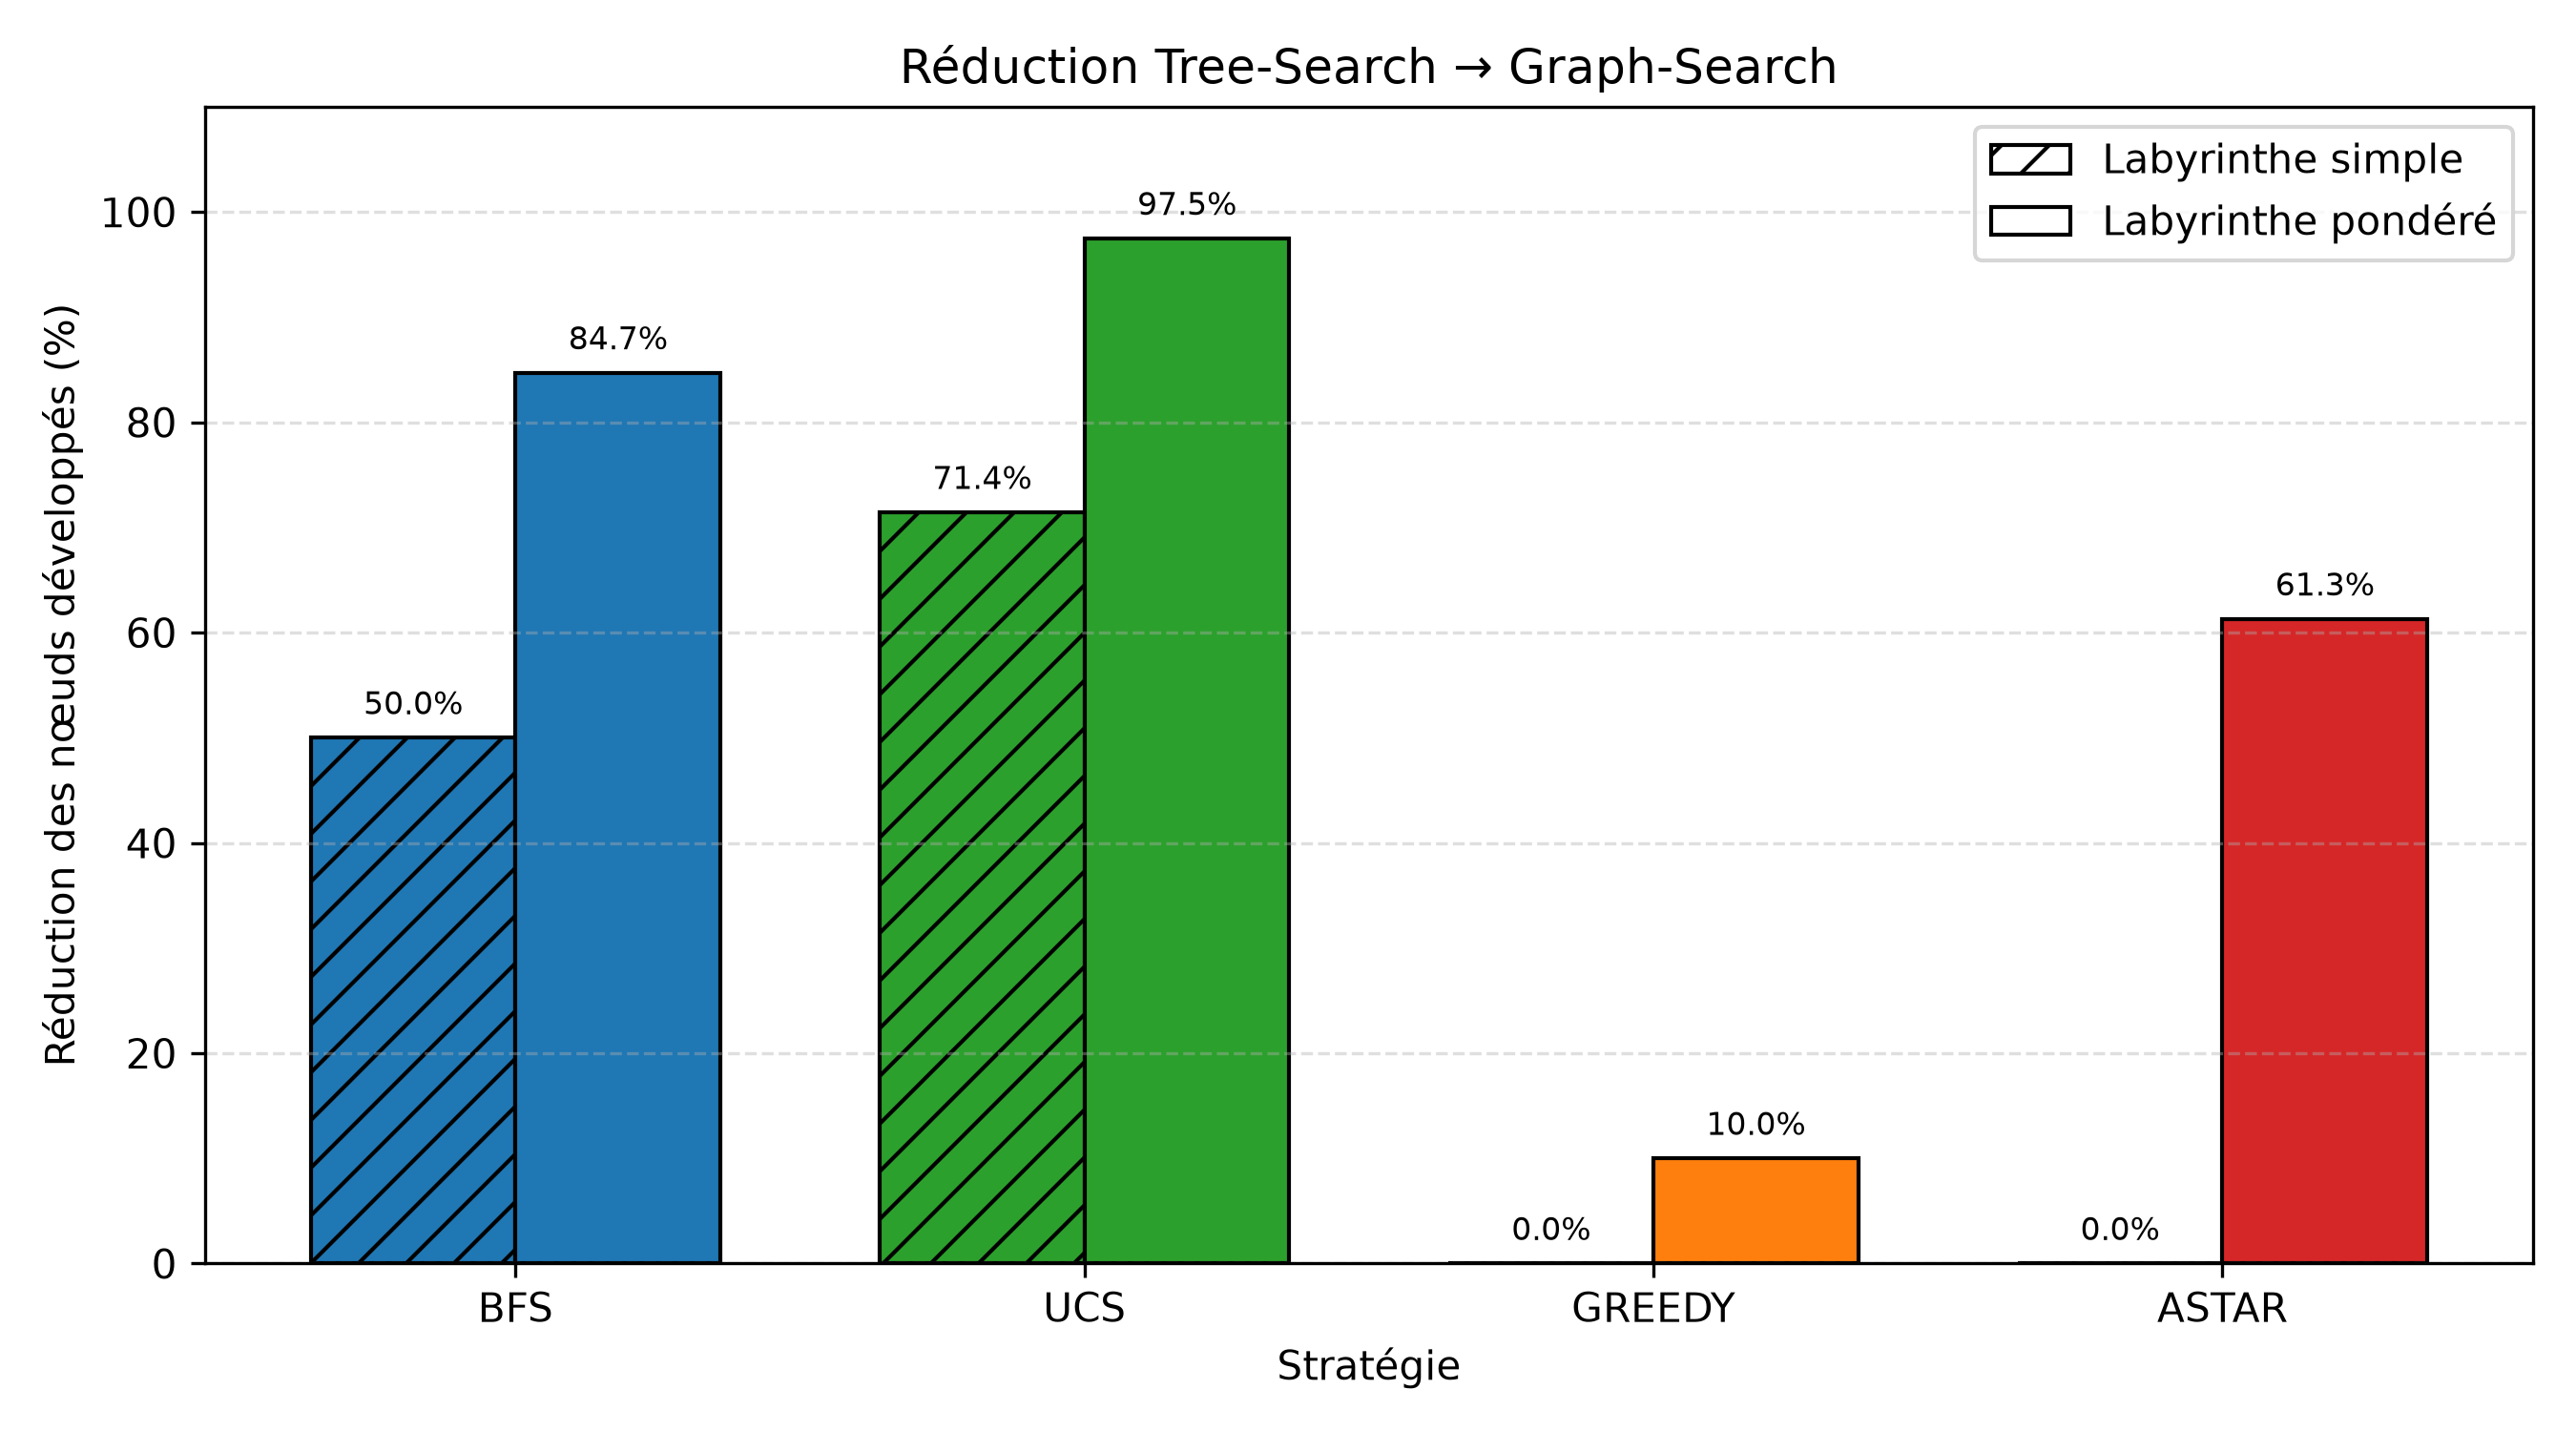
\includegraphics[width=0.78\textwidth]{figures/tree_graph_reduction.png}
\caption{Réduction du nombre de noeuds expansés obtenue avec
\GraphSearch{} sur les deux labyrinthes.}
\label{fig:tree-graph-reduction}
\end{figure}

\subsection{Navigation routière}

Pour le trajet Gatineau--Baie-Comeau, \UCS{} et \AStar{} obtiennent le coût
minimal mesuré de 881,9\,km. \BFS{} et Greedy retournent un trajet de
912,7\,km, de profondeur plus faible. Greedy est le moins expansif avec 6
noeuds, mais ne produit pas le trajet de coût minimal dans cette expérience.

\begin{table}[H]
\centering
\caption{Résultats de navigation de Gatineau à Baie-Comeau en
\GraphSearch{}.}
\label{tab:navigation}
\small
\begin{tabular}{lrrrrrr}
\toprule
\textbf{Stratégie} & \textbf{Coût (km)} & \textbf{Profondeur} &
\textbf{Gén.} & \textbf{Exp.} & \textbf{OPEN max.} & \textbf{Temps (s)} \\
\midrule
BFS & 912,7 & 6 & 69 & 23 & 7 & 0,000081 \\
UCS & 881,9 & 9 & 74 & 25 & 6 & 0,000078 \\
Greedy & 912,7 & 6 & 24 & 6 & 10 & 0,000057 \\
A* & 881,9 & 9 & 48 & 15 & 9 & 0,000112 \\
\bottomrule
\end{tabular}
\end{table}

\begin{figure}[H]
\centering
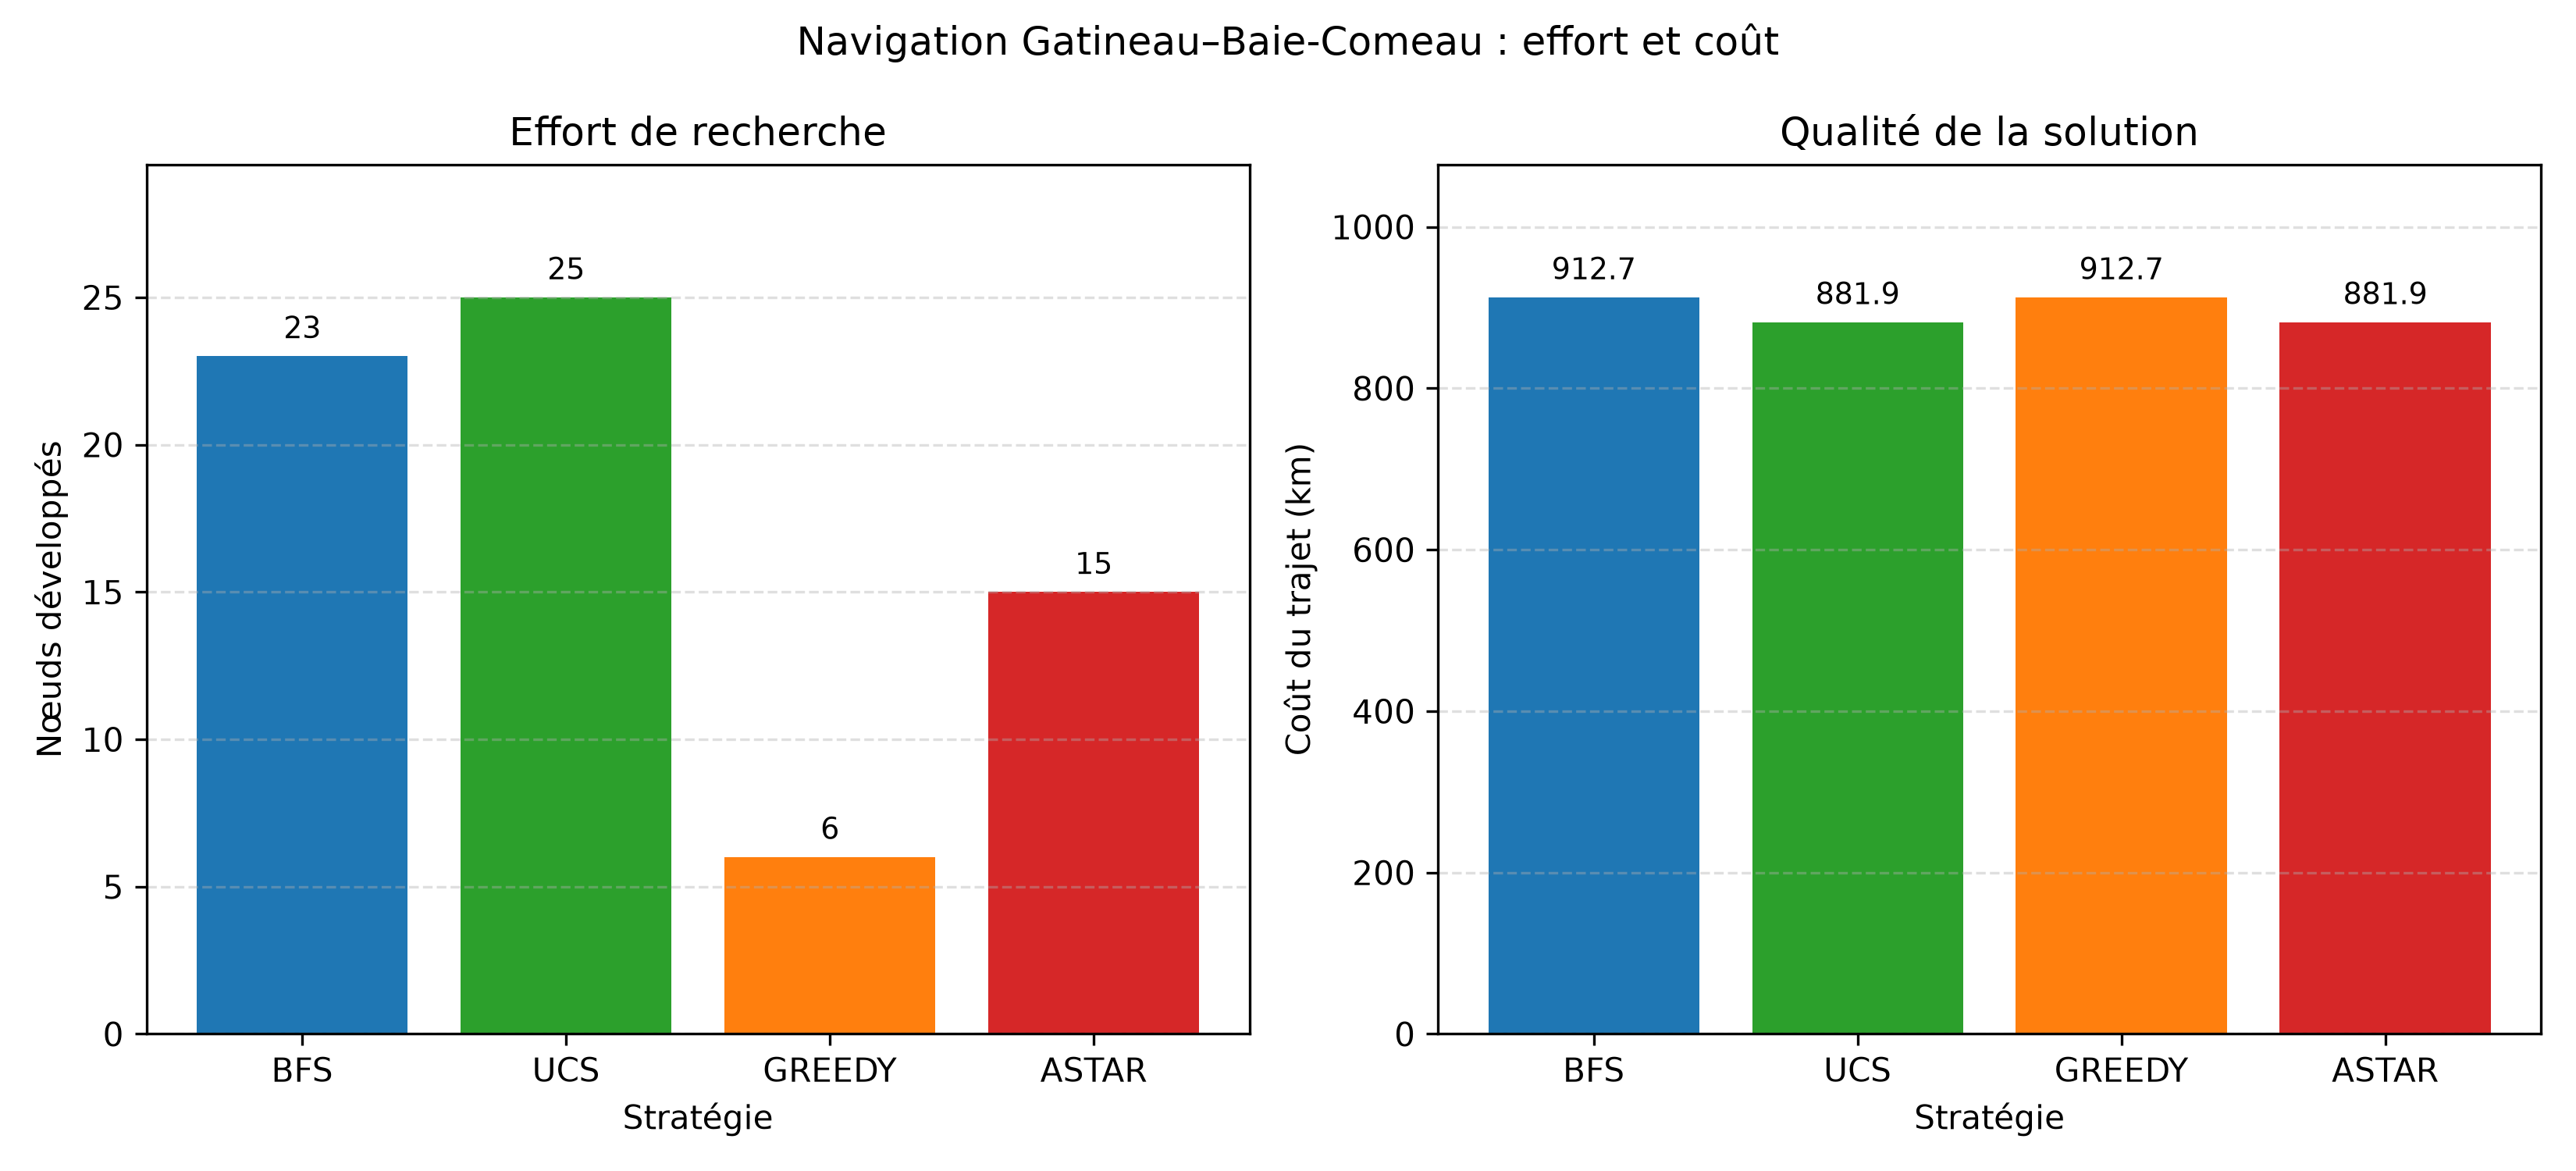
\includegraphics[width=0.92\textwidth]{figures/navigation_strategies.png}
\caption{Effort de recherche et coût de la solution pour le trajet
Gatineau--Baie-Comeau.}
\label{fig:navigation-strategies}
\end{figure}

\subsection{Stratégies sur le 8-Puzzle moyen}

\BFS{}, \UCS{} et \AStar{} trouvent une solution optimale de 28 coups dans
cette instance; \AStar{} développe 1\,440 noeuds contre 171\,028 pour \BFS{}.
Greedy ne développe que 385 noeuds, mais sa solution comporte 48 coups. Ce
résultat illustre le compromis entre l'effort de recherche et la qualité de
solution.

\begin{table}[H]
\centering
\caption{Comparaison des stratégies sur le 8-Puzzle moyen en
\GraphSearch{}.}
\label{tab:npuzzle-strategies}
\small
\begin{tabular}{lrrrrrr}
\toprule
\textbf{Stratégie} & \textbf{Coût} & \textbf{Profondeur} &
\textbf{Gén.} & \textbf{Exp.} & \textbf{OPEN max.} & \textbf{Temps (s)} \\
\midrule
BFS & 28 & 28 & 455\,676 & 171\,028 & 24\,053 & 1,149463 \\
UCS & 28 & 28 & 473\,571 & 177\,134 & 24\,053 & 1,267173 \\
Greedy & 48 & 48 & 1\,052 & 385 & 218 & 0,003184 \\
A* & 28 & 28 & 3\,815 & 1\,440 & 823 & 0,014050 \\
\bottomrule
\end{tabular}
\end{table}

\begin{figure}[H]
\centering
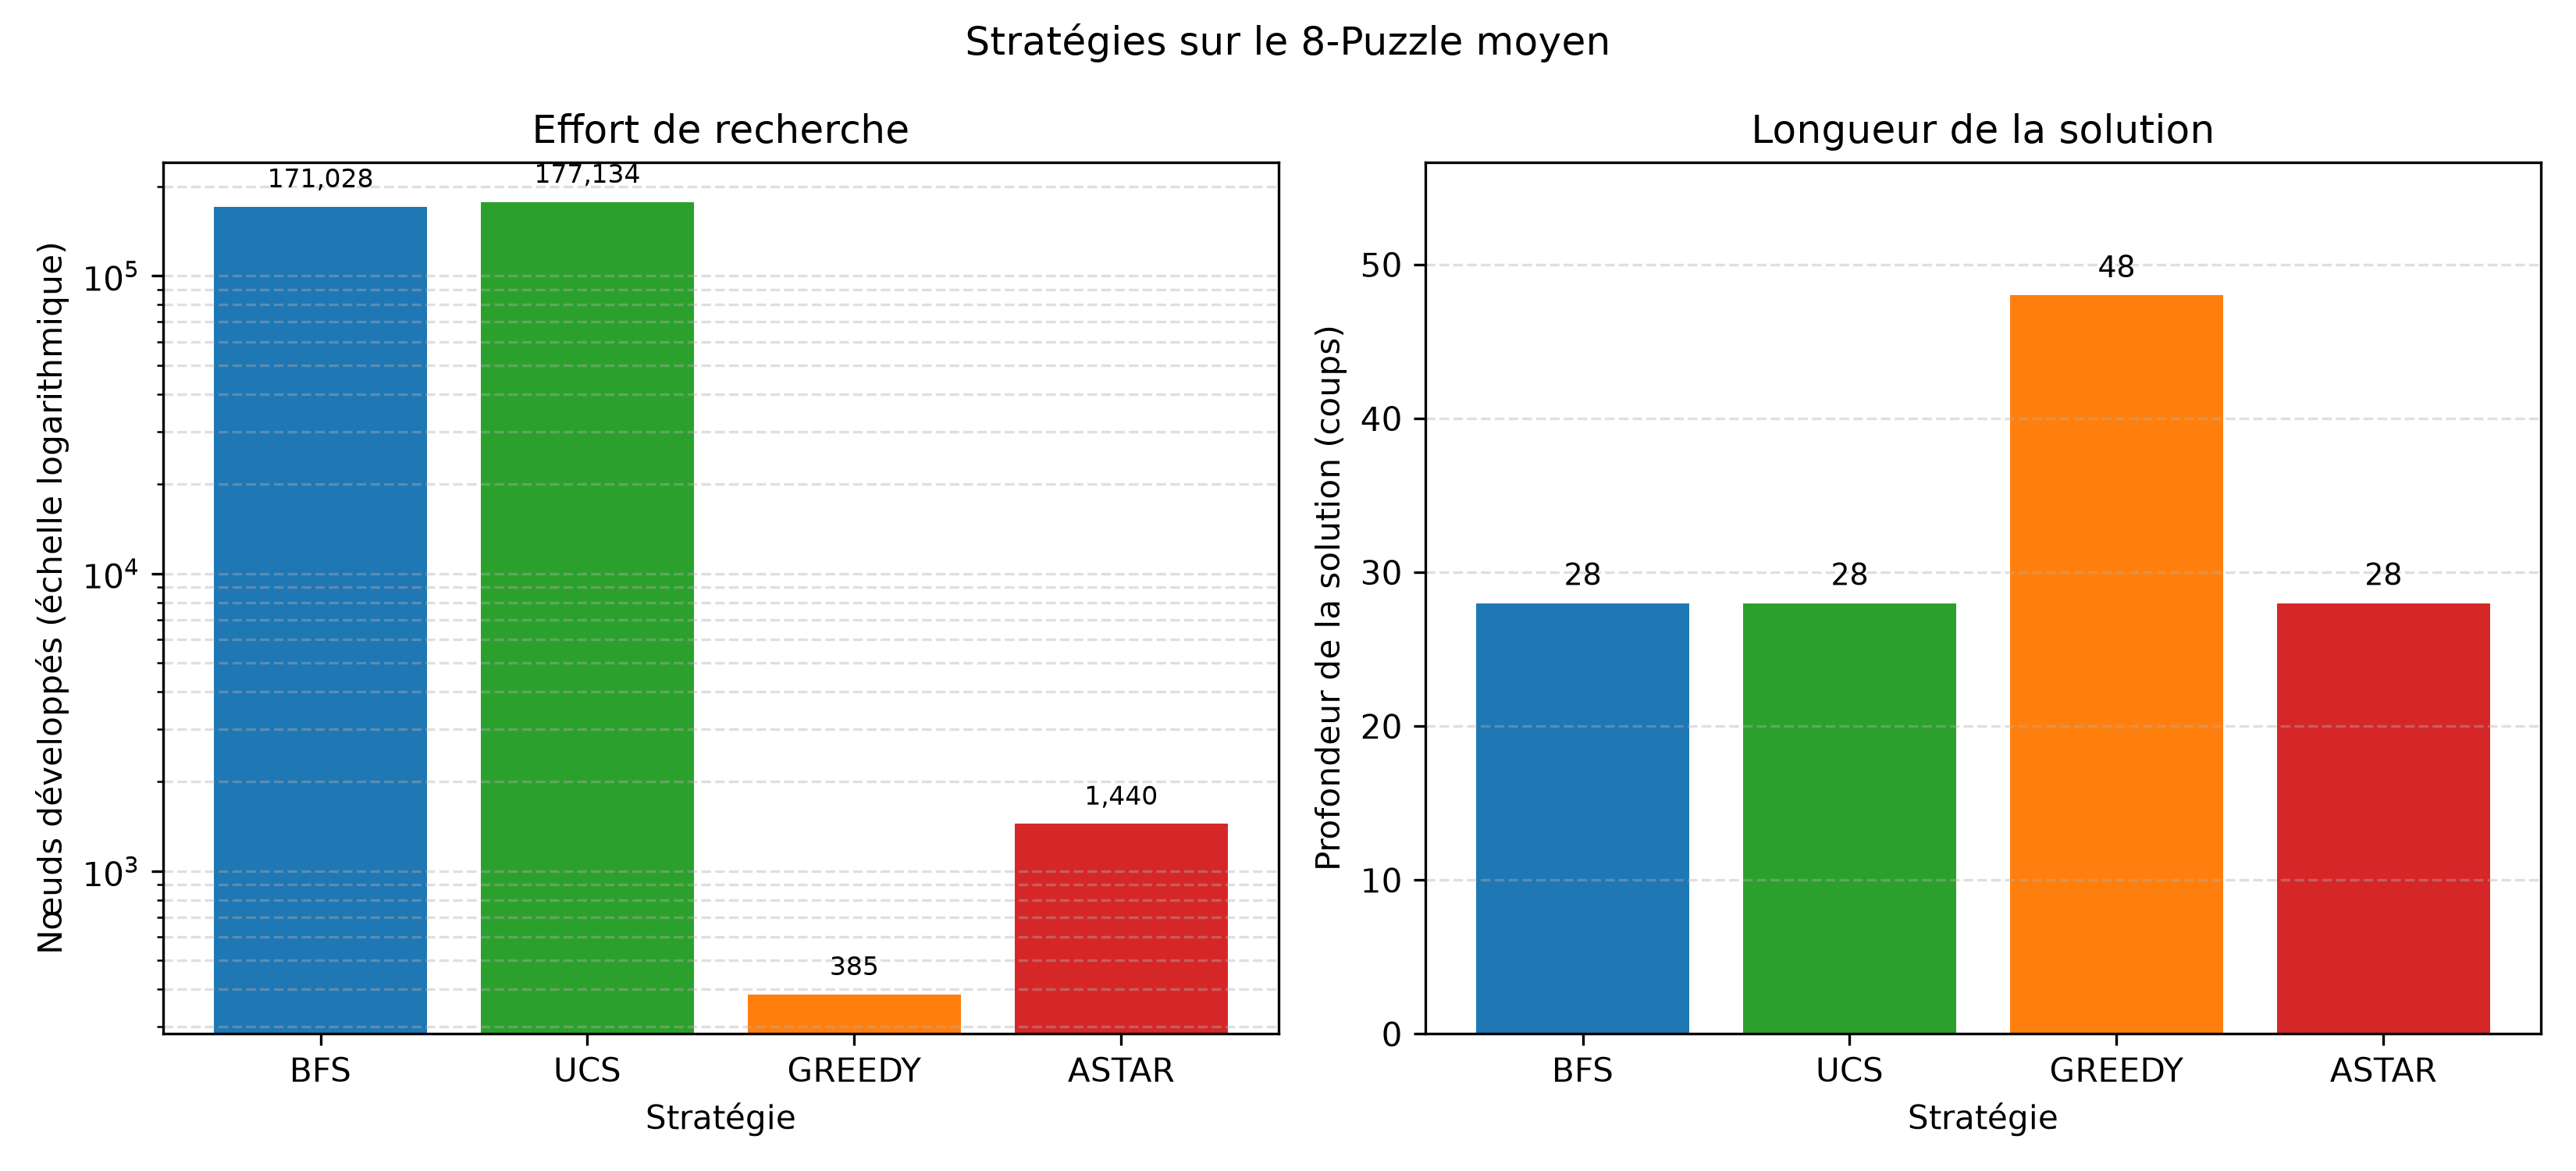
\includegraphics[width=0.92\textwidth]{figures/strategies_npuzzle.png}
\caption{Noeuds expansés et profondeur de solution selon la stratégie sur le
8-Puzzle moyen.}
\label{fig:strategies-npuzzle}
\end{figure}

\subsection{Influence des heuristiques}

Le \cref{tab:heuristique-valeurs} compare les mesures d'\AStar{} sur la même
instance moyenne de 8-Puzzle. Les trois variantes trouvent une solution de coût
28 et de profondeur 28. Manhattan réduit les noeuds expansés de 99,2\,\% par
rapport à $h=0$; l'heuristique des tuiles mal placées les réduit de 66,7\,\%.
Le temps mesuré pour Manhattan est de 0,014178\,s contre 1,388574\,s avec
$h=0$; ces temps ne proviennent que d'une exécution chacun.

\begin{table}[H]
\centering
\caption{Résultats d'\AStar{} selon l'heuristique sur le 8-Puzzle moyen.}
\label{tab:heuristique-valeurs}
\small
\begin{tabular}{lrrrrrr}
\toprule
\textbf{Heuristique} & \textbf{Coût / prof.} & \textbf{Gén.} &
\textbf{Exp.} & \textbf{OPEN max.} & \textbf{Temps (s)} &
\textbf{Réduction exp.} \\
\midrule
$h=0$ & 28 / 28 & 473\,571 & 177\,134 & 24\,053 & 1,388574 & Référence \\
Mal placées & 28 / 28 & 160\,091 & 59\,067 & 22\,060 & 0,592204 & 66,7\,\% \\
Manhattan & 28 / 28 & 3\,815 & 1\,440 & 823 & 0,014178 & 99,2\,\% \\
\bottomrule
\end{tabular}
\end{table}

\begin{figure}[H]
\centering
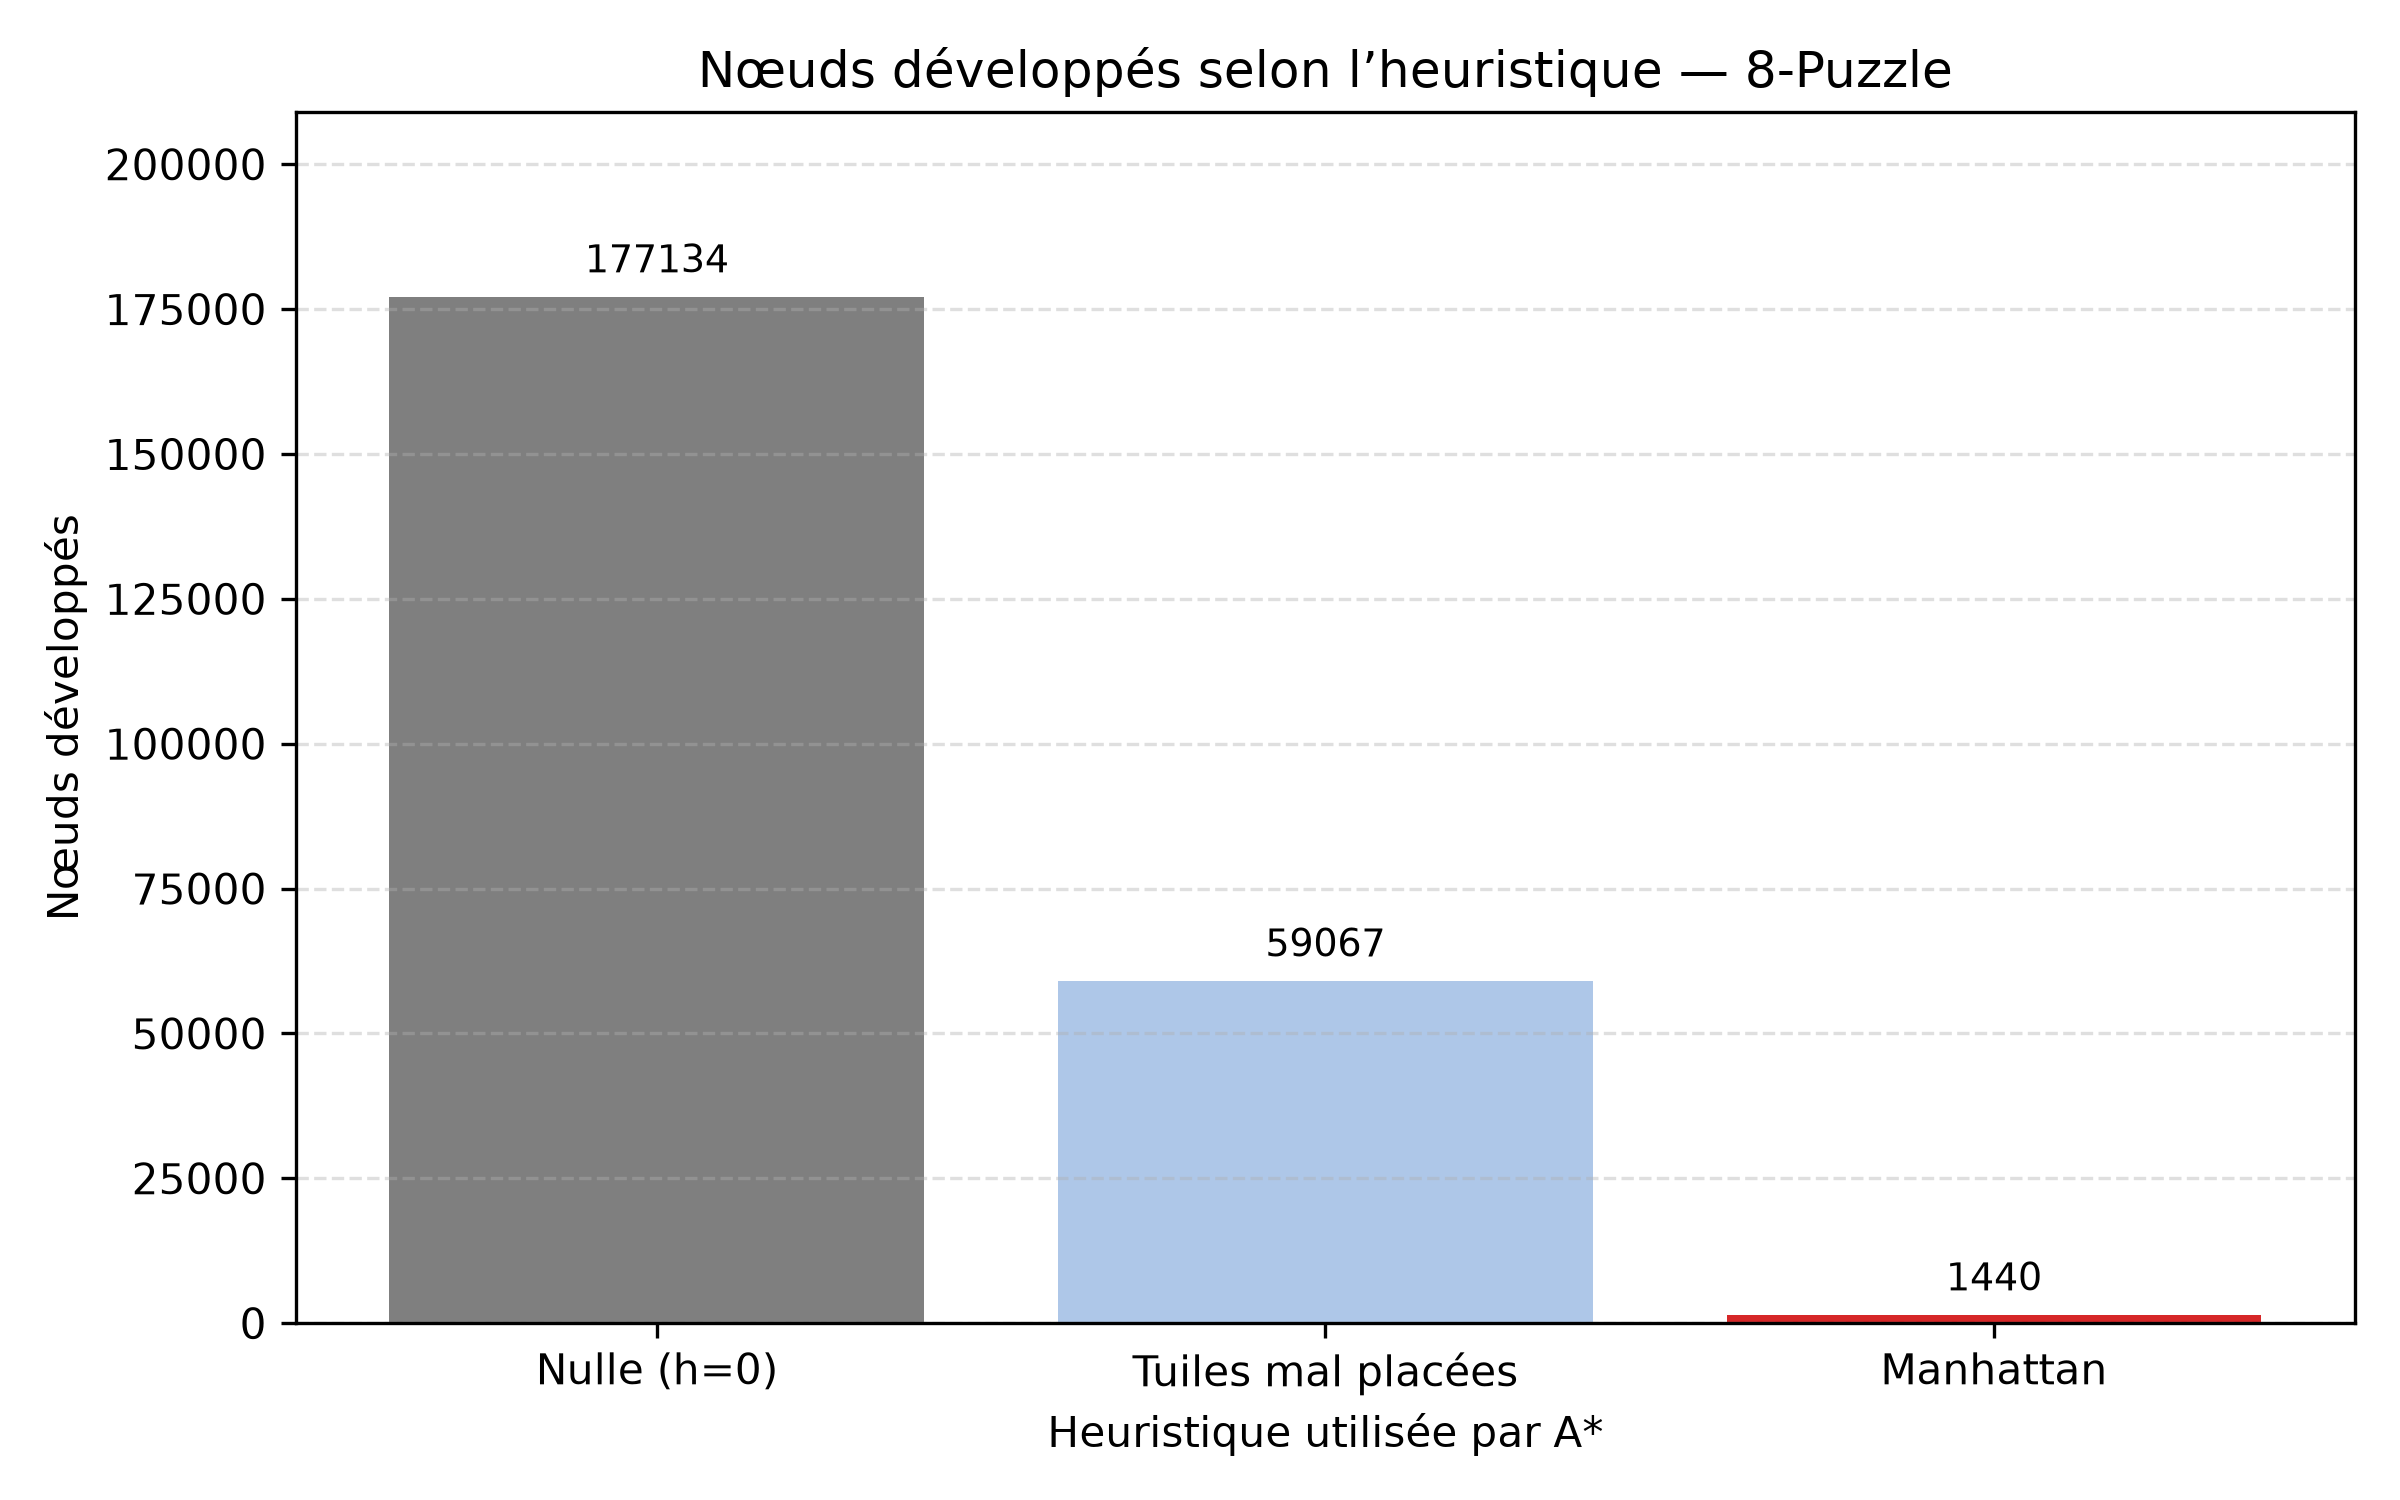
\includegraphics[width=0.82\textwidth]{figures/heuristiques_npuzzle.png}
\caption{Noeuds expansés par \AStar{} selon l'heuristique du 8-Puzzle.}
\label{fig:heuristiques-npuzzle}
\end{figure}

\begin{figure}[H]
\centering
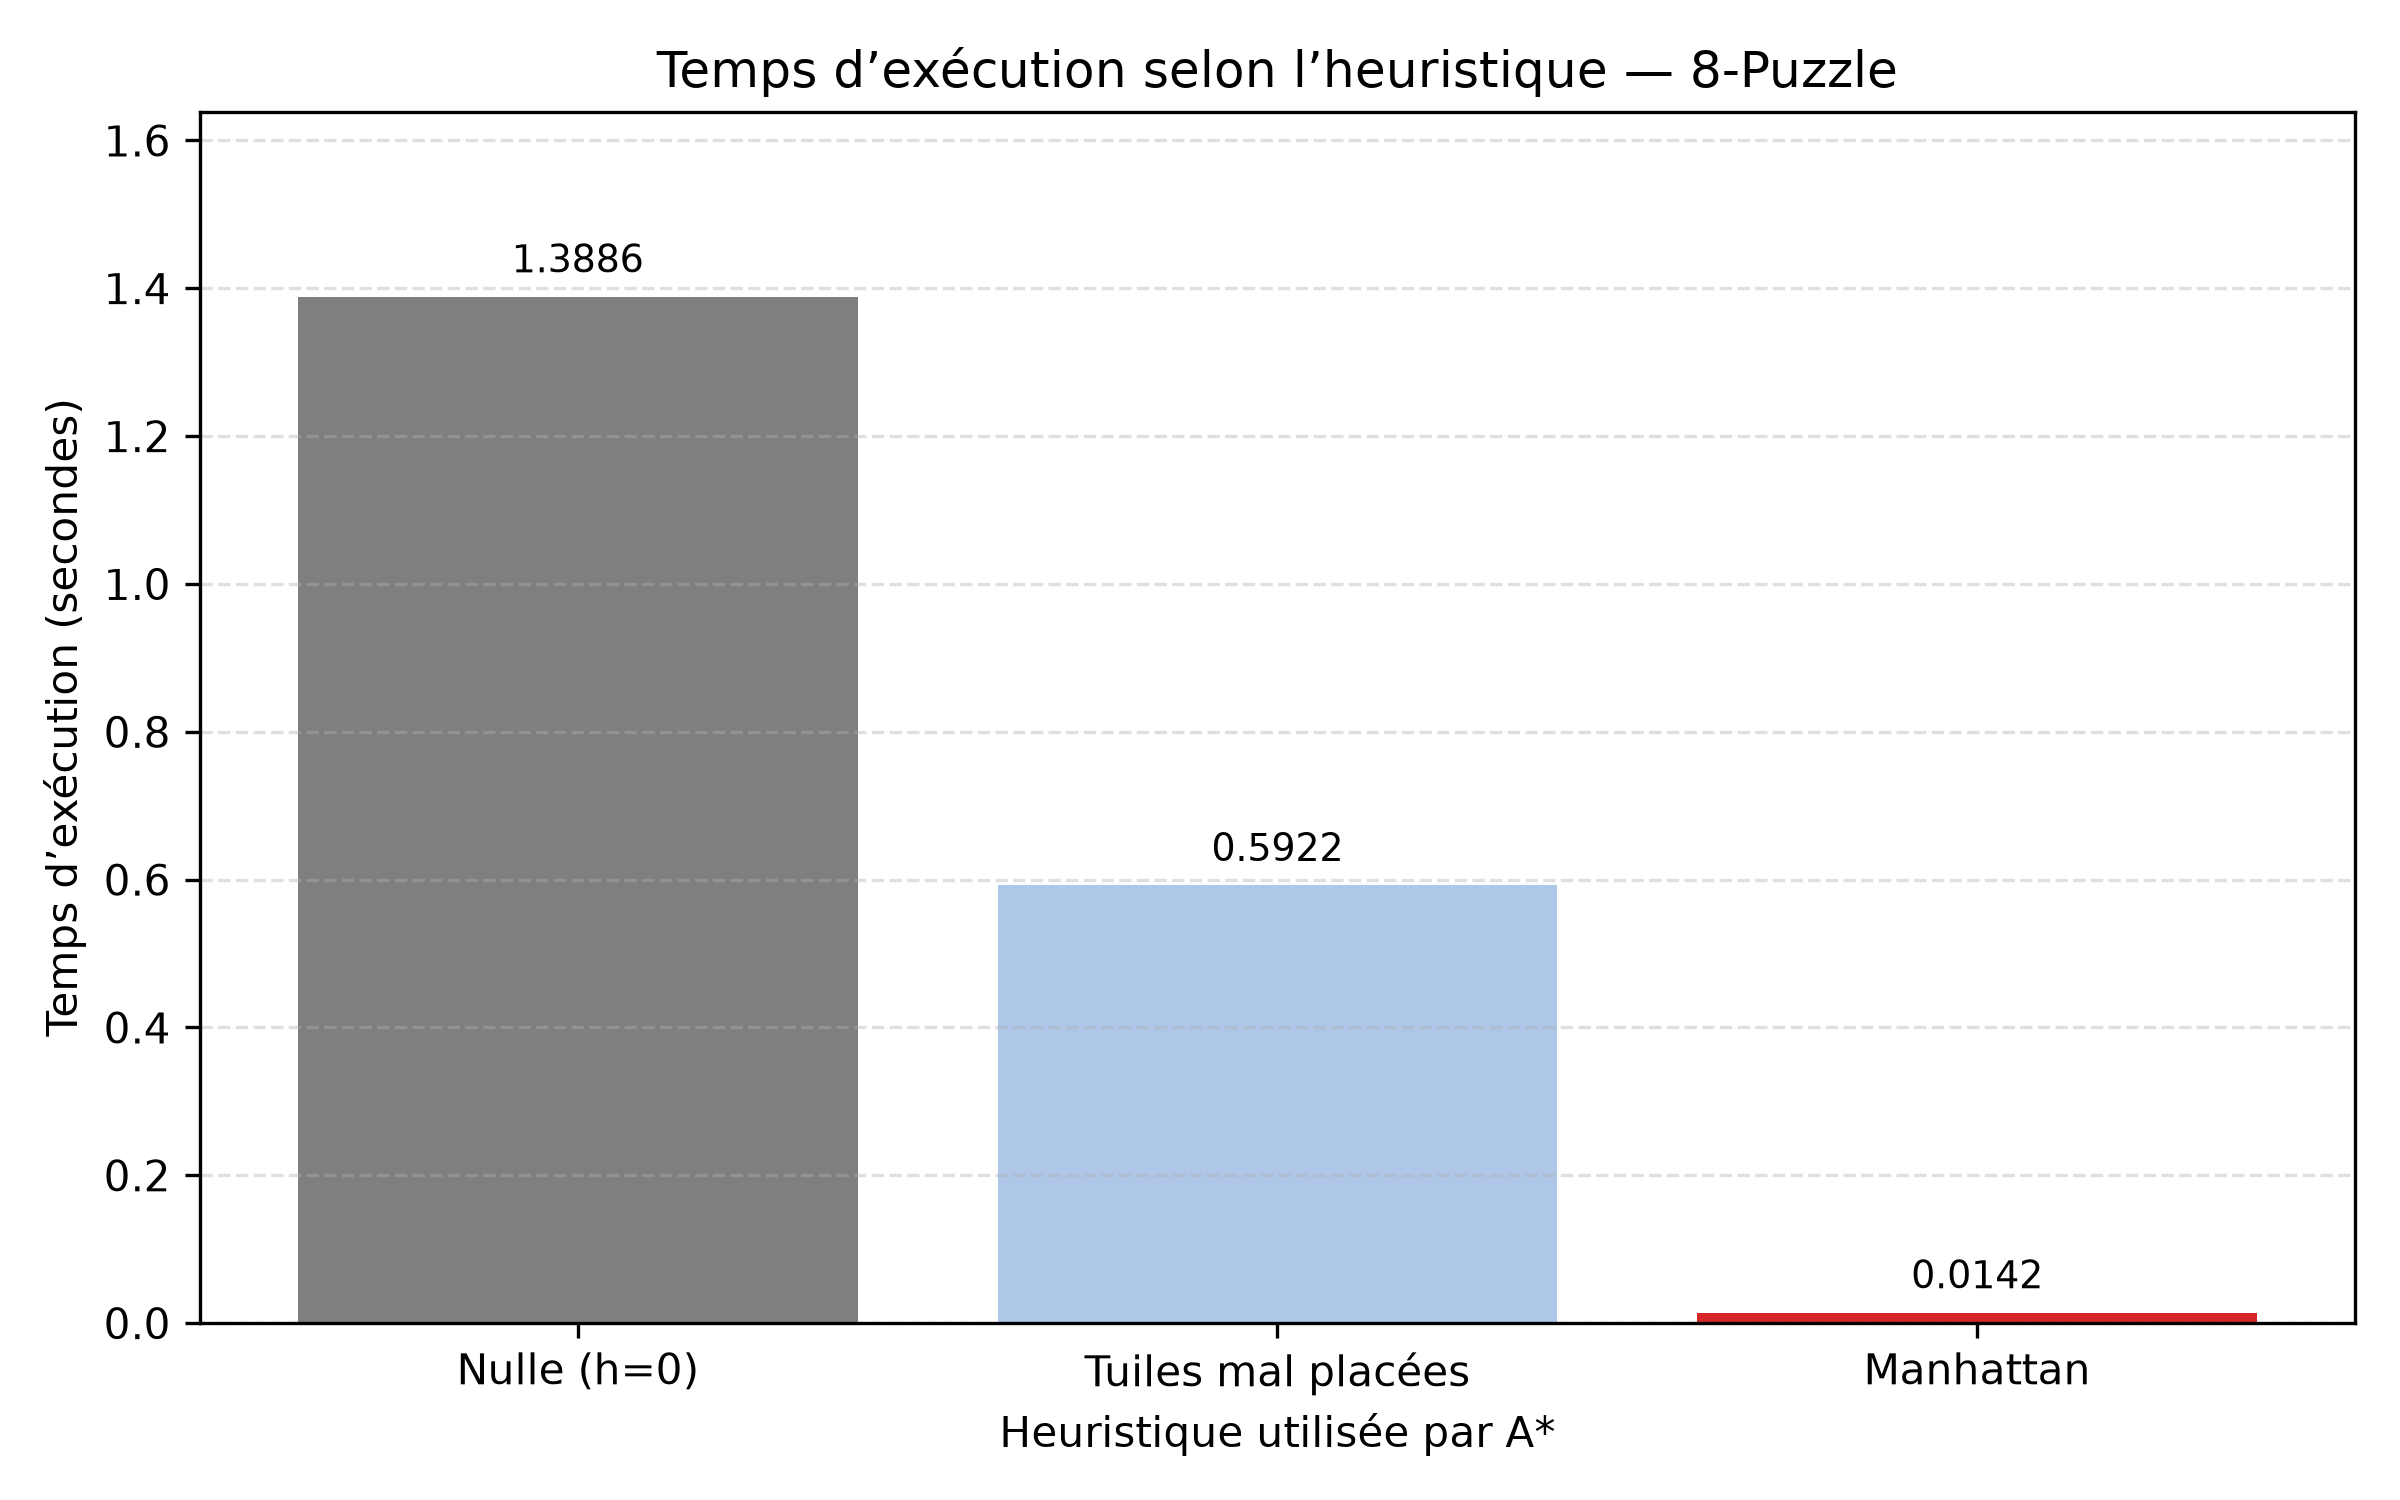
\includegraphics[width=0.82\textwidth]{figures/heuristiques_temps.png}
\caption{Temps mesuré par \AStar{} selon l'heuristique du 8-Puzzle.}
\label{fig:heuristiques-temps}
\end{figure}

\begin{figure}[H]
\centering
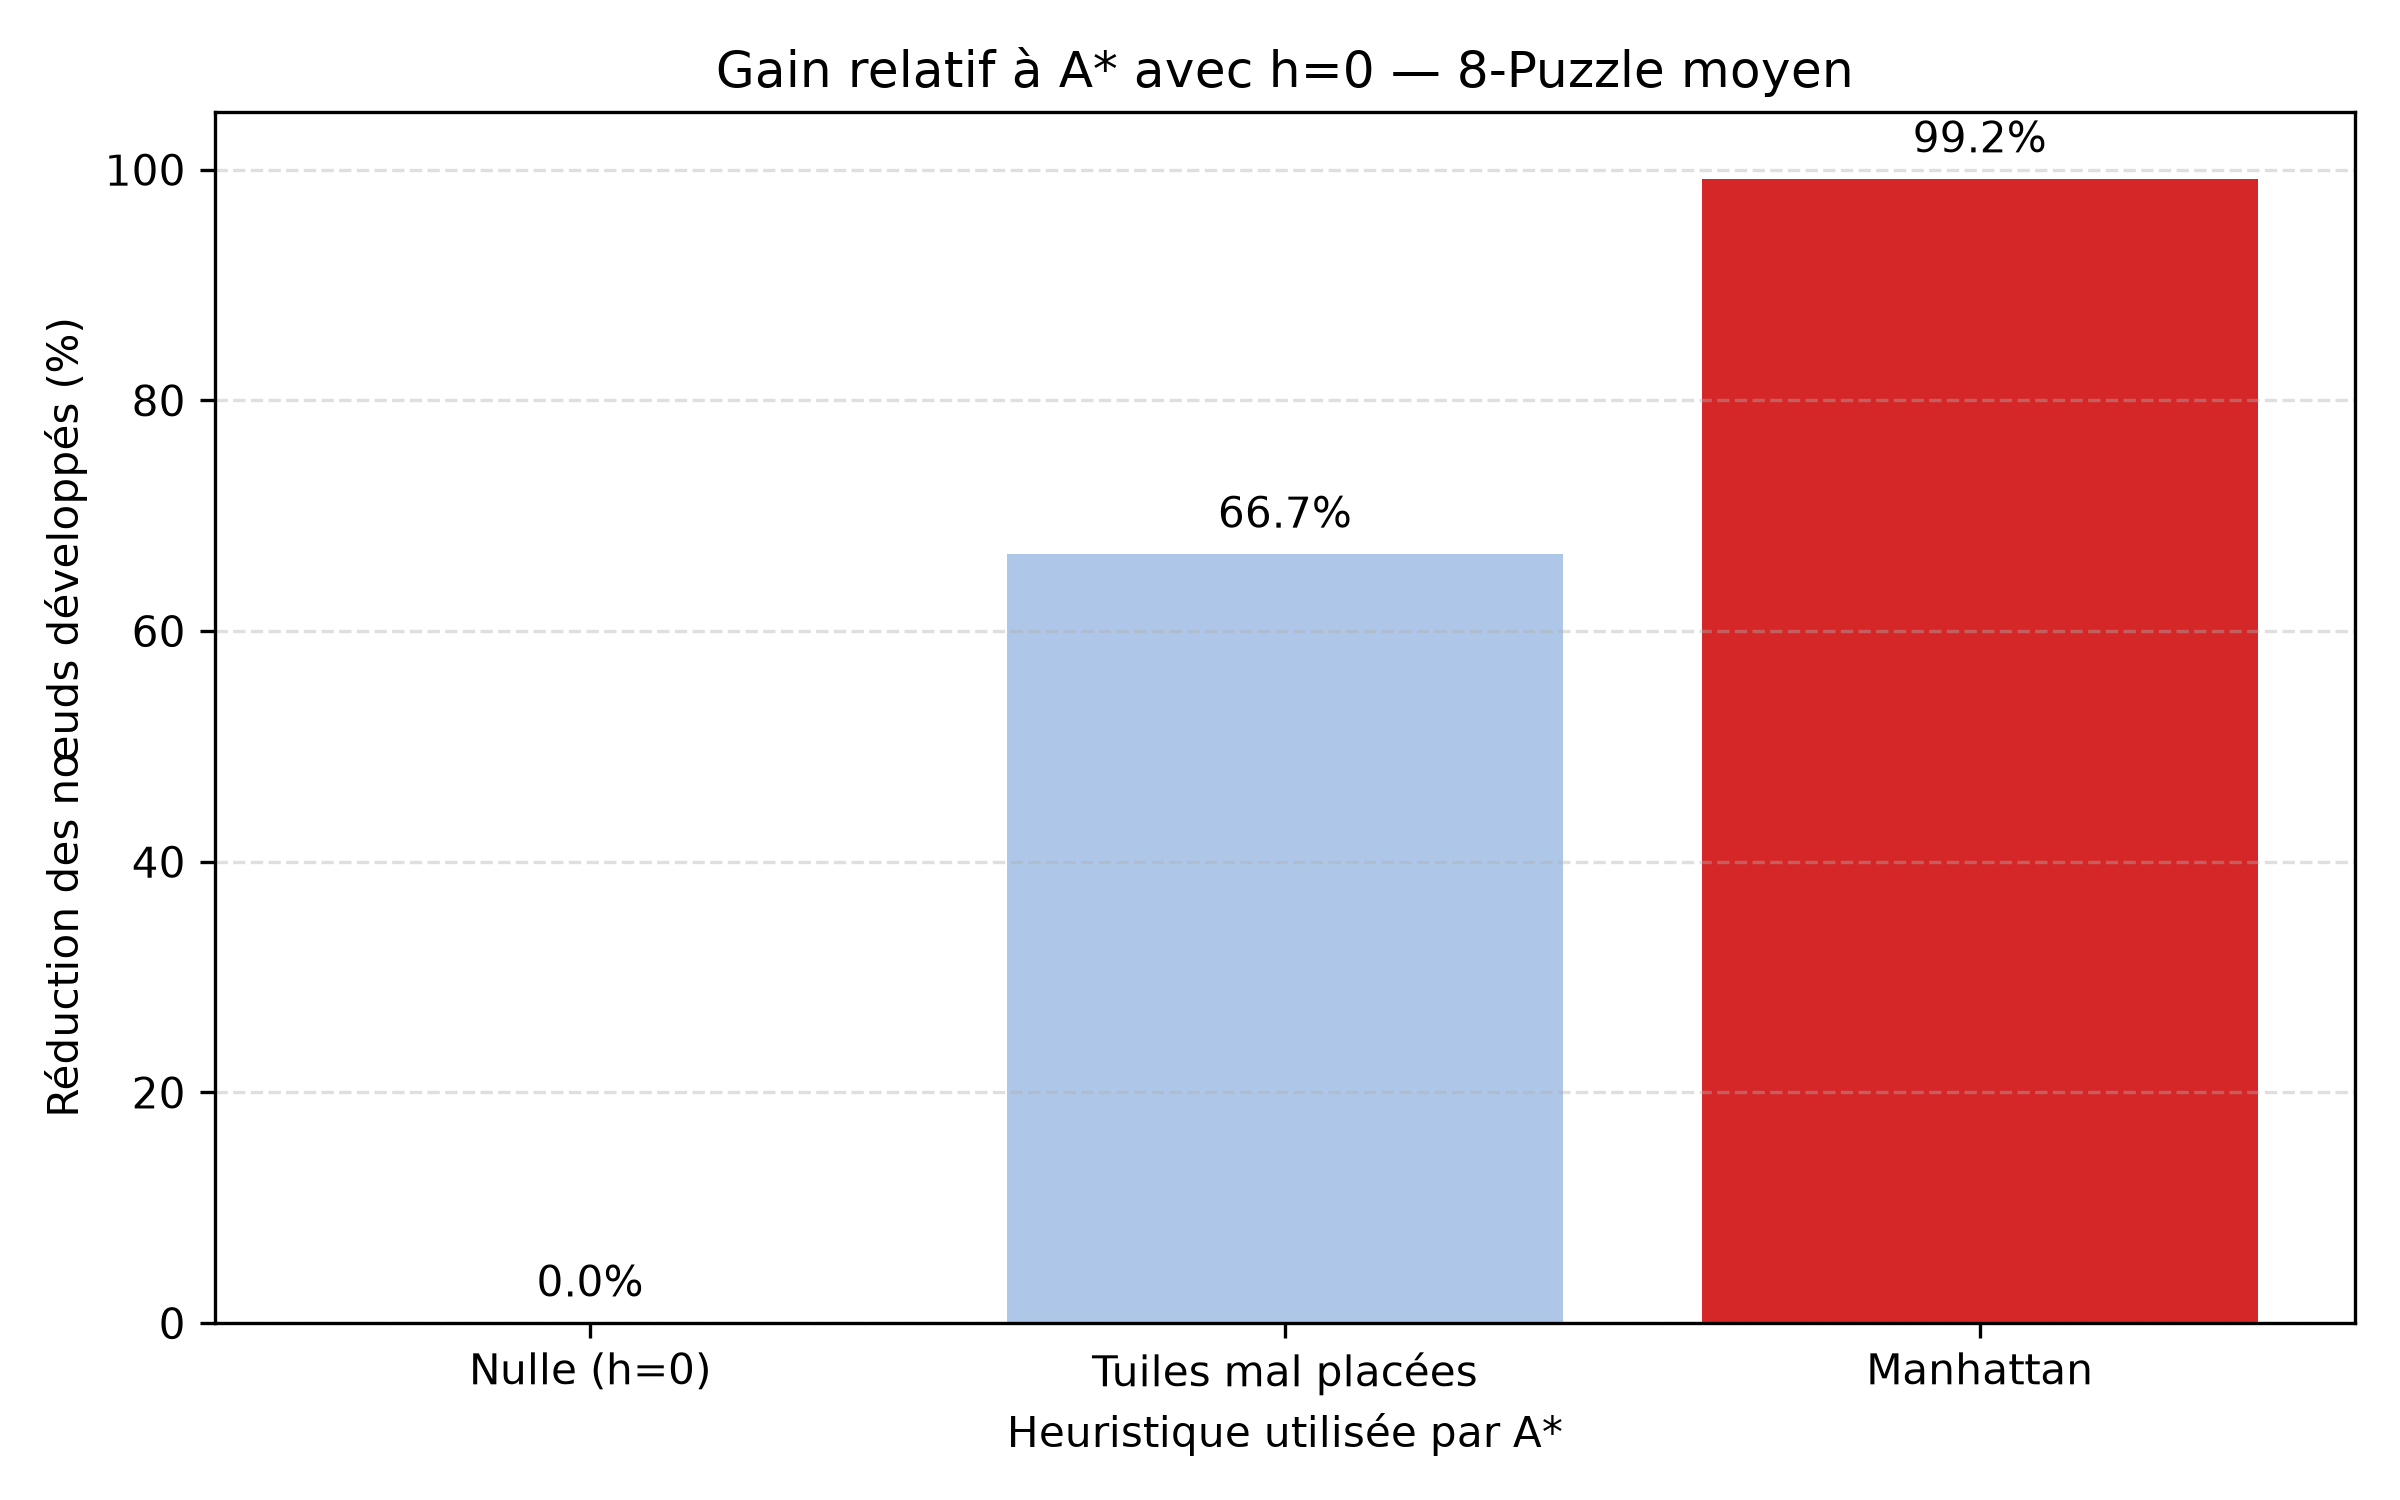
\includegraphics[width=0.78\textwidth]{figures/heuristiques_gain.png}
\caption{Réduction des noeuds expansés par rapport à \AStar{} avec
$h=0$.}
\label{fig:heuristiques-gain}
\end{figure}

\subsection{Jeu arithmétique : cas résolu et cas impossible}

Pour la cible 24, les quatre stratégies trouvent une solution en trois
opérations. Pour la cible 99 avec les nombres $1,1,1,1$, aucune solution n'est
trouvée et la frontière est entièrement épuisée. Chaque stratégie génère 97
noeuds et en développe 20 pour établir cet échec.

\begin{table}[H]
\centering
\caption{Résultats du jeu arithmétique en \GraphSearch{}.}
\label{tab:arithmetique-resultats}
\scriptsize
\begin{tabular}{llrrrrrr}
\toprule
\textbf{Instance} & \textbf{Stratégie} & \textbf{Résolue} &
\textbf{Coût / prof.} & \textbf{Gén.} & \textbf{Exp.} &
\textbf{OPEN max.} & \textbf{Temps (s)} \\
\midrule
Cible 24 & BFS & Oui & 3 / 3 & 881 & 114 & 321 & 0,007114 \\
Cible 24 & UCS & Oui & 3 / 3 & 1\,523 & 434 & 385 & 0,009120 \\
Cible 24 & Greedy & Oui & 3 / 3 & 558 & 284 & 45 & 0,004525 \\
Cible 24 & A* & Oui & 3 / 3 & 558 & 284 & 45 & 0,003879 \\
Cible 99 & BFS & Non & -- & 97 & 20 & 12 & 0,000560 \\
Cible 99 & UCS & Non & -- & 97 & 20 & 12 & 0,000545 \\
Cible 99 & Greedy & Non & -- & 97 & 20 & 10 & 0,000886 \\
Cible 99 & A* & Non & -- & 97 & 20 & 10 & 0,001107 \\
\bottomrule
\end{tabular}
\end{table}

\begin{figure}[H]
\centering
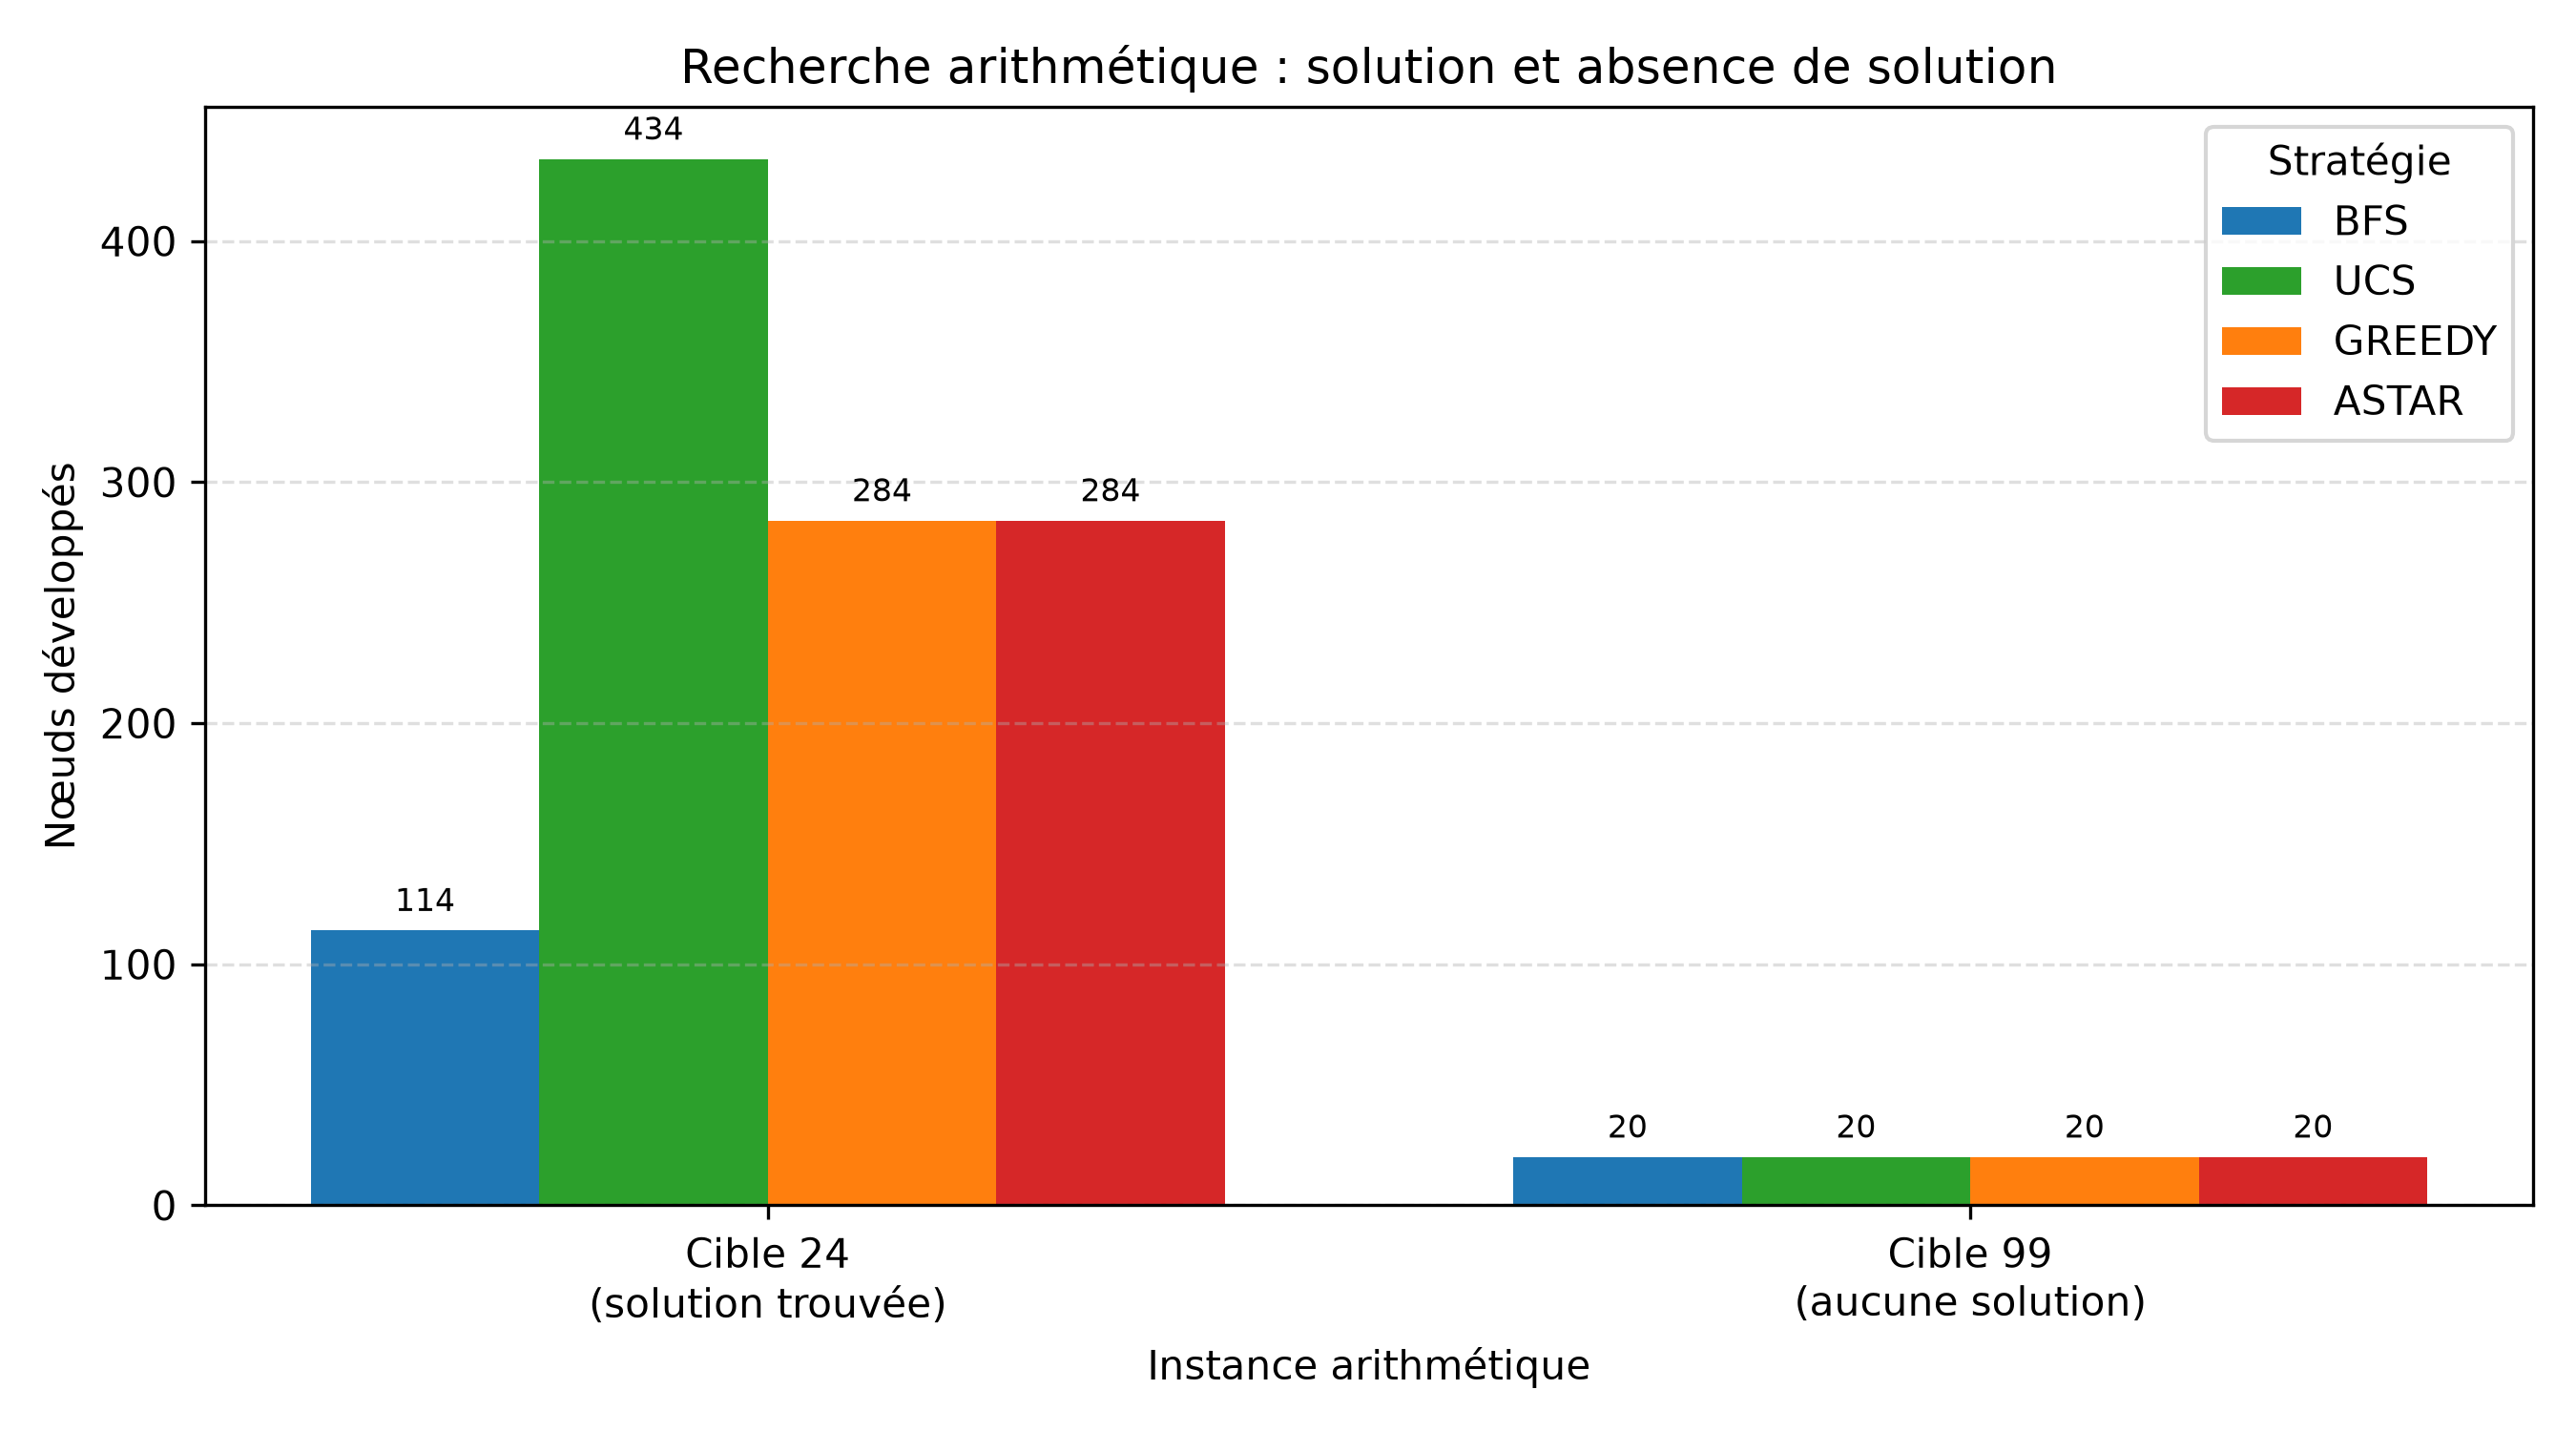
\includegraphics[width=0.82\textwidth]{figures/arithmetique_resultats.png}
\caption{Noeuds expansés pour le cas arithmétique résolu et le cas sans
solution.}
\label{fig:arithmetique-resultats}
\end{figure}

\subsection{Portée des résultats}

Ces mesures correspondent à un benchmark ciblé et ne remplacent pas les
expériences plus larges éventuellement présentées dans d'autres documents.
L'instance de labyrinthe pondéré testée donne le même coût à toutes les
stratégies; elle ne suffit donc pas à démontrer à elle seule que \BFS{} peut
être sous-optimale en présence de coûts variables. De même, une seule mesure
de temps par configuration ne permet pas d'établir une moyenne ou un intervalle
de confiance. Ces limites doivent être prises en compte dans l'interprétation.
